\section{Matrix Element Method}
\label{sec:mem}

\subsection{Hypothesis testing}

\subsection{Optimal test statistic}
\label{sec:test_statistic}

\subsection{Description of MEM}

The MEM is a multivariate analysis technique in which we directly compute the per-event probability density that depends on model parameters $\vec{\theta}$

\begin{equation}
P_{\vec{\theta}}(\vec{y}) = \frac{1}{\sigma}
\frac{\mathrm{d}\sigma_{\vec{\theta}}(\vec{y})}{\mathrm{d}\vec{y}}
\end{equation}
and use it in hypothesis testing as component of the test statistic. Through the differential cross section, the MEM explicitly depends on $\vec{y} = (\tilde{p}_{i \in \mathrm{jets}}, \tilde{p}_{i \in \mathrm{leptons}}, \dots)$, the vector containing the detector-level 4-momenta of the reconstructed particles, in particular, jets and leptons. The differential cross-section(\cref{eq:diff_cross_section}) depends on the squared matrix element $|\mathcal{M}^2|$ that we use to directly take into account the dynamics of the relevant underlying processes. The kinematics of the $2 \rightarrow n$ scattering process are encoded in the $n$-body phase space element(\cref{eq:n_body_phase_space}), where the delta function enforces the conservation of momentum between the initial and final state particles.

\begin{equation}
\label{eq:diff_cross_section}
\mathrm{d}\sigma_{\vec{\theta}} = \frac{(2\pi)^4 |\mathcal{M}_{\vec{\theta}}|^2}{4 \sqrt{(q_1 \cdot q_2)^2 - m_1 m_2}} \times
\mathrm{d}\Phi_n(q_1 + q_2; p_1, \dots, p_{n})
\end{equation}

\begin{equation}
\label{eq:n_body_phase_space}
\mathrm{d}\Phi_n = \delta^4 (q_1 + q_2 - \sum_{i=1}^n p_i) \prod_{i=1}^n \frac{\mathrm{d}^3 p_i}{(2\pi)^3 2 E_i}
\end{equation}
We have to consider several additional effects:
\begin{itemize}
\item We cannot directly observe the momenta of the initial state particles $q_1$ and $q_2$ in a proton-proton collision.
\item We do not measure the momenta of the neutrinos or jets that do not pass a transverse momentum threshold and the detector has a finite energy resolution.
\item We do not know which of the observed jets are matched to which partons.
\item The non-zero final transverse momentum caused by large-angle initial state radiation, spoiling the momentum balance in \cref{eq:n_body_phase_space}.
\end{itemize}

To address the first issue, we need to use parton density functions $g(x_{1,2})$ to weight the differential cross-section, integrating over the momentum fractions $x_{1,2} = E_{q_{1,2}}/E_{\mathrm{beam}}$.

In order to take into account detector effects, we integrate over unmeasured or poorly measured quantities using a transfer function $W(\vec{y}, \vec{p})$.
The transfer function relates final state parton-level quantities $\vec{p}$ to measurable quantities on the detector level $\vec{y}$ and encodes our knowledge about detector resolution or reconstruction efficiencies.

The question of jet-to-parton matching is addressed by summing over the $N_a$ possible permutations of jet-to-parton matching, which depends on assumptions about the process and the number of observed final state particles and is encoded in the exact factorized form of the transfer function $W(\vec{y}, \vec{p})$.

Finally, the modelling of the non-zero transverse recoil $\vec{\rho}_T = -\sum_{i=1}^n \vec{p}_{i,T}$ is treated empirically using a transfer function $\mathcal{R}(\tilde{\vec{\rho}}_T, \vec{\rho}_T)$ determined on simulation that relates the parton-level transverse momentum of the system $\vec{\rho}_T$ to the observed recoil $\tilde{\vec{\rho}}_T$. 

The evaluation of $|\mathcal{M}_{\vec{\theta}}|^2$ requires full knowledge of the initial and final state momenta, as well as the parameters of the model, summarized in $\vec{\theta}$. In particular, the parameters of the model contain the hypothesis $\mathcal{H} \in \{\ttH, \ttbb\}$ about the underlying process and the assumptions about which of the partons formed reconstructed jets $\mathcal{C}$, such that $\vec{\theta} = (\dots, \mathcal{H}, \mathcal{C})$. In the case of \ttH with the top quark pair decaying semileptonically $\ttH \rightarrow (\ell^- \bar{\mathrm{\nu}}_\ell) \mathrm{b}\ (\mathrm{q} \mathrm{q}' \bar{\mathrm{b}})\ (\mathrm{b} \bar{\mathrm{b}})$, we may consider the fully reconstructed category where all 6 of the final state partons are reconstructed as jets, denoted as $2_W 2_H 2_t$, the case where one of the quarks from the hadronic decay $\mathrm{W} \rightarrow \mathrm{q} \mathrm{q}'$ is out of acceptance, denoted as $1_W 2_H 2_t$ and so forth, such that $\mathcal{C}_{\mathrm{SL}} \in \{ 2_W 2_H 2_t, 1_W 2_H 2_t, \dots \}$. The number of unknown quantities to be integrated over depends on the reconstruction category $\mathcal{C}$, as described in detail in the next section. 
Thus, the per-event probability density takes the form
\begin{align}
\label{eq:mem_definition}
P(\vec{y}, \vec{\theta}) &= \sum_{k=1}^{N_a} \int \frac{\mathrm{d}x_1 \mathrm{d}x_2}{2 x_1 x_2 s} \int \prod_{i=1}^{n} \frac{\mathrm{d}^3 p_i}{(2\pi)^3 2 E_i} \\
&\times \delta^4 (q_1 + q_2 - \sum_{i=1}^n p_i)\\
&\times g(x_1) g(x_2) \\ 
&\times \mathcal{R}(\tilde{\vec{\rho}}_T, \vec{\rho}_T) \\ 
&\times |\mathcal{M}_{\vec{\theta}}(q_1, q_2, p_1, \dots, p_n)|^2 \\
&\times W(\vec{y}, \vec{p})
\end{align}

After having been first proposed for reconstructing events with missing momentum\cite{Kondo1988}, the MEM has been used in Tevatron for Higgs boson searches\fix and a precise measurement of the top quark mass\cite{D0topmass2004}. After first phenomenological studies showed that MEM could be used effectively for \ttH in a multi-parton final state\cite{Artoisenet2013}, it has been used in searches for \ttH by the CMS and ATLAS experiments in Run I of the LHC\fix. The MEM approach is closely related to MELA\cite{Gao} that has been extensively used in $\mathrm{H} \rightarrow \mathrm{ZZ} \rightarrow 4\mathrm{l}$ searches and $J^P$ measurements, however, in MELA, unreconstructed particles and transfer functions are not considered and the matrix elements have generally simple analytical forms.
In the following, we discuss in detail the implementation and improvements that were made to the MEM for Run II.

\subsection{Implementation}
\label{sec:mem_implementation}
In the case of semileptonic or dileptonic \ttH final state, the observables $\vec{y}$ consist of the energies (or equivalently transverse momenta) and the directions of the jets, the momenta of the charged leptons and the measured recoil of the system $\tilde{\vec{\rho}}_T$. As \cref{eq:mem_definition} needs to be integrated numerically, we first need to define it explicitly in terms of variables that are convenient and suitable for integration, namely energies, solid angles and combinations of invariant masses. The Jacobian transformation can be done analytically for both the top and antitop quarks and is of the form shown in \cref{eq:phase_space_jacobian}.
\fix
\begin{align}
\label{eq:phase_space_jacobian}
\fix
\end{align}

The scattering amplitude written as $|\mathcal{M}(\vec{p})|^2$ depends only on particle momenta, hence it is implied to be summed over spin and colour states. Furthermore, we treat the production and decay of the top quarks, W and Higgs bosons in the narrow-width approximation\cite{Berdine2007}, meaning we factorize the production and decay of these particles, as seen in \cref{eq:scattering_nwa}.

\begin{align}
\label{eq:scattering_nwa}
|\mathcal{M}_{\ttH \rightarrow (qq'b) (qq'\bar{b}) (b\bar{b})}|^2 &= |\mathcal{M}_{gg \rightarrow \ttH}(g_1, g_2, t, \bar{t}, h)|^2 \\
&\times \prod_{r = t,\bar{t}} \bigl[ \frac{\pi}{m_t \Gamma_t} \delta(t^2 - m_t^2) |\mathcal{M}_t(q,\bar{q},b)|^2 \bigr]_r \\
&\times \frac{\pi}{m_t \Gamma_t} \delta(h^2 - m_H^2) |\mathcal{M}_H(b,\bar{b})|^2
\end{align}

The decay amplitude of the top quark, assuming NWA for the W-boson, is given in \cref{eq:decay_top} and for the $\mathrm{H} \rightarrow \mathrm{b}\bar{\mathrm{b}}$ in \cref{eq:decay_higgs}.

\begin{equation}
\label{eq:decay_top}
FIXME
\end{equation}

\begin{equation}
\label{eq:decay_higgs}
FIXME
\end{equation}

\subsubsection{Transfer functions}
\label{sec:transfer_functions}

The transfer function $W(\vec{y} | \vec{p})$ maps a point $\vec{p} \in \Omega$ in the phase space to a point $\vec{y} \in \mathcal{A}$ in the space of reconstructed variables and it is ensured to be normalized to unity using \cref{eq:transfer_normalization}, which means that in an observable fiducial region, a phase space point has an efficiency $\epsilon(\vec{p}) \leq 1$ to be reconstructed. We note that since the same transfer functions are applied for all hypotheses, the choice of transfer functions ultimately affects the model sensitivity, but not the correctness, that is, we are not introducing any bias into the analysis with our assumptions.

\begin{equation}
\label{eq:transfer_normalization}
\int \mathrm{d}\vec{y}~W(\vec{y} | \vec{p}) = 1
\end{equation}

We can make further progress by factorizing the transfer function in terms of individual reconstructed objects, the jets and leptons:
\begin{equation}
W(\vec{y} | \vec{p}) = \prod_{i\in \mathrm{jets}} W(E_i, \vec{e}_i | E_{q_i}, \vec{e}_{q_i})
\prod_{i\in \ell^\pm} W(E_i, \vec{e}_i | E_{\ell_i}, \vec{e}_{\ell_i}) = \prod_{i \in \mathrm{jets}} W_{i,j} \prod_{i \in \ell^\pm} W_{i,\ell},
\end{equation}
where $q_i$ ($\ell_i$) is shorthand for the quark (charged lepton) assumed to give rise to the $i$-th measured jet (charged lepton). If we are dealing with indistinguishable objects such as jets, we have to sum over all possible ways of matching the detector-level and parton-level objects, such that
\begin{equation}
\label{eq:tf_combination_sum}
W_{i,j} \propto \sum_{q_i \in \mathrm{quarks}} W(E_i, \vec{e}_i | E_{q_i}, \vec{e}_{q_i}).
\end{equation}
In particular, we make no assumption on jet charge, therefore, to assign out of 4 reconstructed b-jets 2 to the quarks from $\Hbb$, we have $4!/2!2! = 6$ combinations. Without distinguishing between $\mathrm{b}$ and $\bar{\mathrm{b}}$, we have a further $2!/1!1!$ ways of assigning the b-tagged jets to bottom quarks from the top or antitop quarks. We describe the approach taken to reducing the number of required combinations further in \cref{sec:event_interpretation}.

Lepton energies and directions are measured with an order of magnitude higher resolution than jet energies, therefore we assume those to be perfectly measured so that their transfer functions are Dirac delta functions.
Furthermore, we assume that the jet energy and angular transfer functions can be factorized such that
\begin{equation}
W(E_i, \vec{e}_i | E_{q_i}, \vec{e}_{q_i}) = W(E_i | E_{q_i}) \times W(\vec{e}_i | \vec{e}_{q_i}).
\end{equation}
With these assumptions, the transfer function for observed particles reduces to a product of $W(E_i | E_{q_i})$ over the jets.

For light partons, the quark energy transfer functions are modelled by a Gaussian function, shown in \cref{eq:single_gaussian}, 

\begin{equation}
\label{eq:single_gaussian}
W(p_{T,j} | p_{T,\mathrm{gen}}) = p_0 \exp{\biggl(\frac{p_{T,j} - p_1}{p_2}\biggr)^2},
\end{equation}

whereas for bottom quarks as double-Gaussians to account for the low-energy tails resulting from semi-leptonic decays of B hadrons, shown in \cref{eq:double_gaussian}.

\begin{equation}
\label{eq:double_gaussian}
W(p_{T,j} | p_{T,\mathrm{gen}}) = p_0 \biggl[0.7\exp{\biggl(\frac{p_{T,j} - p_1}{p_2}\biggr)^2} + 0.3\exp{\biggl(\frac{p_{T,j} - p_3}{p_2+p_4}\biggr)^2}\biggr]
\end{equation}

The parameters of these transfer functions are derived from MC simulation, assuming that they depend on quark energy, direction and flavour. We extract the transfer functions from a \ttbar MC sample by matching the generator-level partons geometrically to jets using $\Delta R(q,j) < 0.3$ and performing fits of the $W(p_{T,j}|p_{T,q})$. We fit the parameters $p_0 \dots p_4$ of \cref{eq:single_gaussian} and \cref{eq:double_gaussian} in bins of $p_{T,q}$, $|\eta_{q}|$ and flavour $\mathrm{f}\in{\mathrm{l}, \mathrm{b}}$. Additionally, in order to have a smooth dependence of the transfer functions on \ptgen~, we fit polynominals to the per-bin parameters $p_n(\ptgen|\eta_{q},\mathrm{f})$.

\fix plot of transfer function fits


As we are considering both SL and DL \ttH decays, the reconstruction resolution of \MET has to be taken into account via a transfer function. We model it via a Gaussian with a resolution $\sigma_{MET}^2 = 30\GeV$, which is of similar magnitude to detector resolution and does not affect the results significantly.
It is possible to evaluate the covariance matrix of \MET~on an event-by-event basis and thus take into account the correlation between the $\MET_x$ and $\MET_y$ components in the MEM\cite{cms_htautau}. This would mean that the full \MET~transfer function is a multivariate gaussian
\begin{equation}
W_{\MET}(\vec{\rho}_T | \sum_k \vec{p}_k) = \frac{1}{2\pi |\Sigma|^{1/2}} \exp \biggl[ -\frac{1}{2} (\vec{\rho}_T - \sum_k \vec{p}_k)^T \Sigma^{-1} (\vec{\rho}_T - \sum_k \vec{p}_k)\biggr],
\end{equation}
where we currently have assumed $\Sigma = \sigma_{\MET} \mathbf{I}$.

\subsubsection{Lost quarks}
\label{sec:lost_quarks}

In Run II, we have extended the MEM to deal with scenarios where one or more of the quarks from the underlying $pp \rightarrow \ttH(\rightarrow \bb),\ttbb$ processes is not reconstructed due to either being out of the geometrical detector acceptance $|\eta_j| > \eta_{\mathrm{cut}}$ or due to hadronising into a jet that is below an experimental threshold $E_j < E_{\mathrm{cut}}$.
Formally, we extend the space of observables $\vec{y} \rightarrow \vec{y}' = (\vec{y}, (E_q, \vec{e}_q)_{q \in \mathrm{lost}})$ and the per-event matrix element probability
\begin{equation}
P(\vec{y}) \rightarrow P'(\vec{y}') = \frac{1}{\sigma'} \frac{\mathrm{d} \sigma_i}{\mathrm{d}\vec{y} \prod_{q\in\mathrm{lost}} \mathrm{d}E_j \mathrm{d}\vec{e}_j}
\end{equation}
and integrate out the unobserved quantities:
\begin{equation}
P(\vec{y}) = \int_{\mathcal{O}'} \bigl[ \prod_{q \in \mathrm{lost}} \mathrm{d}E_q \mathrm{d}\vec{e}_q \bigr] P'(\vec{y}').
\end{equation}
This integral over the lost quarks simplifies to
\begin{equation}
P(\vec{y}) = \int \dots \prod_{q\in\mathrm{lost}} \biggl[ \int_{|\eta_q| \leq \eta_{\mathrm{cut}}} \mathrm{d}\Omega_q \epsilon(E_q, \eta_q) + \int_{|\eta_q| > \eta_{\mathrm{cut}}} \mathrm{d}\Omega_q \dots \biggr] \times \dots
\end{equation}
where $\epsilon(E_q, \eta_q)$ is the probability for a quark of energy $E_q$ at a pseudorapidity $\eta_q$ to hadronise to a jet below the energy threshold $E_{\mathrm{cut}}(\eta_q)$ and thus fail to be reconstructed:
\begin{equation}
\epsilon(E_q, \eta_q) = \int_0^{E_{\mathrm{cut}}(\eta_q)} \mathrm{d}E_j W(E_j | E_q).
\end{equation}
This means that for every lost quark, we add 2 integration variables through $\mathrm{d}\Omega_q$, as well as an extra combination of choosing which of the quarks did not produce a jet. The flexibility afforded by this technique, which makes the MEM applicable for cases where we may not always reconstruct the exact multi-particle final state, thus comes at a computational cost which is evaluated in \cref{sec:mem_computational}.

\subsubsection{Treatment of QCD radiation}

The MEM as formulated above does not account for QCD radiation, which at the LHC can be substantial. In particular, we estimate using simulation that \fix\% of \ttHbb events are reconstructed with 7 or more jets, whereas the hard interaction produces only 6 partons at LO. Additionally, ISR that is not reconstructed as jets also affects the kinematics of the event with an unknown component in the final momentum balance. We have implemented and compared several alternative techniques that extend the MEM to final states with additional radiation.

First, to deal with unreconstructed ISR, we note that momentum balance can be restored by performing a Lorentz boost with $\beta(\vec{p}_k) = (\sum_k p_{k,x}, \sum_k p_{k,y}, \beta_z)$ in the transverse plane, such that a Born-like configuration with a null transverse momentum is achieved. The longitudinal component $\beta_z$ of the boost is in principle unknown and should be integrated out. However, we find that it can be ignored by setting $\beta_z = 0$, since it corresponds to different values for gluon fractions $x_{1,2}$ which are found not to affect the performance of the matrix element significantly. This simple treatment of ISR kinematics is necessary to evaluate the LO matrix element with proper momentum balance, but it does not take into account the dynamics of ISR production nor the properties of QCD radiation in general.

A possible step forward would be to use additional matrix elements with more final state partons to take into account extra jets. In particular, for events with one extra jet, we can use the $\mathrm{pp} \rightarrow \ttHbb + \mathrm{g}$ matrix element. For a semileptonic top decay, we would thus have 7 final state partons that need to be matched to 7 jets. This approach has the advantage of not making the assumption that the extra jet arises necessarily from ISR, but is instead a full treatment of the $2 \rightarrow 7$ scattering with perturbation theory. However, the additional computational complexity is significant, especially if (anti)quark diagrams are included as well.

Sudakov reweighting allows us to approximate the effects of ISR in the scattering amplitude in terms of splitting functions derived from QCD. At detector level, the Sudakov factor is approximated by a log-normal transfer function of the form
\begin{equation}
W(p_T) = \frac{1}{\sqrt{2\pi} \sigma p_T} \exp \biggl[ \frac{-(\ln{p_T/1~\mathrm{GeV}} - \mu)^2}{2\sigma^2}\biggr]
\end{equation}
that estimates the probability of the parton-level transverse momentum $p_T$ resulting in an observed recoil $\rho_T$ below an experimental threshold $\rho_{T,0} < 30~\mathrm{GeV}$, taking into account detector resolution. Here the the values $\mu = 4.1$ and $\sigma = 1.35$ are estimated from MC simulation and the unknown momentum ISR momentum $p_T$ is integrated out. We have implemented this empirical factor and compared it with the nominal LO MEM. In case a significant missing transverse momentum is observed, a separate double-gaussian transfer function would be appropriate. However, since we independently have to consider a transfer function for the MET due to the presence of neutrinos, the modelling of ISR can be absorbed in it.

\fix Plot of nominal, Sudakov, Recoil, additional diagrams, ttH only.

\subsubsection{Event interpretations}
\label{sec:event_interpretation}

The scattering amplitude $|\mathcal{M}_{\vec{\theta}}|$ depends on the assumed process $\mathcal{H}$ and the interpretation of the event $\mathcal{C}$. Various interpretations are possible, depending on the number of charged leptons and jets. First, the number of charged leptons fixes the choice of the top decay amplitudes between the semileptonic, dileptonic or all-hadronic. This in turn determines the number of quarks in the final state. Depending on the nature and number of the observed jets, we consider 4 classes of event interpretations:
\begin{itemize}
\item \textbf{Fully reconstructed events}: In this case $N_{\mathrm{jets}} = N_{\mathrm{quarks}}$, such that each each quark is associated with a jet. This is the standard case.
\item \textbf{Over-reconstructed events}: If $N{\mathrm{jets}} > N_{\mathrm{quarks}}$, we may choose up to $N_{\mathrm{quarks}}$ jets out of the set of reconstructed jets, such that each quark is associated with a jet and the left-over jets are ignored. In doing this, we sum over the possible choice of jets using the combinatorial approach of the MEM
\item \textbf{Over-reconstructed events with an ISR interpretation}: If $N_{\mathrm{jets}} = N_{\mathrm{quarks}} + 1$, we may act as above, but choose to interpret the extra jet as arising from gluon radiation in the initial state using the LO diagrams $\ttH + \mathrm{g}$ and  $\ttbb + \mathrm{g}$ in a full MEM approach by extending the reconstructed phase space $\vec{y}$. Due to the higher complexity of the involved diagrams, this approach is computationally more costly than the above, but includes information on the dynamics and kinematics of the additional jet.
\item \textbf{Partially-reconstructed events}: In case $N_{\mathrm{jets}} < N_{\mathrm{quarks}}$, we treat a number of quarks as lost and integrate over their directions as described in \cref{sec:lost_quarks}. This allows the MEM to be used as a discriminator on a wider range of events, but we may also apply this hypothesis in case we suspect some jets may be mismeasured and not correspond to the underlying hard interaction, thus integrating them out
\end{itemize}

In the most general case, we could evaluate all possible event interpretations and use them as a combined event discriminator that makes maximal use of kinematics and our hypotheses about what processes are likely. However, this is computationally prohibitive, requiring many numerical integrals per event, each taking $\mathcal{O}(10^1)\dots \mathcal{O}(10^3)$ seconds on a modern CPU. Therefore, it is necessary to restrict the interpretation space using MC simulation, comparing the expected performance of various interpretation strategies and choosing one providing an acceptable trade-off between discriminator performance and computational cost. We list the interpretations that were considered in \cref{tab:event_interpretation_list}.

\begin{table}[h!]

\begin{center}
\caption{The detailed event interpretations for semileptonic and dileptonic \ttH (\ttbb) events. We consider cases where up to 2 light quarks may be lost and independently one of the bottom quarks from top or Higgs decay. For the fully-reconstructed semileptonic case, we also consider the ISR-modified interpretation.}
\label{tab:event_interpretation_list}
\begin{tabular}{c|ccc}
\hline
interpretation & bottom quarks & light quarks & description \\
\hline
SL $2_{\mathrm{W}} 2_{\mathrm{h}} 2_{\mathrm{t}}$ & 4 & 2 & fully-reconstructed semileptonic \\
SL $1_{\mathrm{W}} 2_{\mathrm{h}} 2_{\mathrm{t}}$ & 4 & 1 & $(l \nu_{l}' \mathrm{b})_{\mathrm{t}} (\cancel{\mathrm{q}} \mathrm{q}' \bar{\mathrm{b}})_{\bar{\mathrm{t}}} (\mathrm{b} \bar{\mathrm{b}})_{\mathrm{h}}$ \\
SL $0_{\mathrm{W}} 2_{\mathrm{h}} 2_{\mathrm{t}}$ & 4 & 0 & $(l \nu_{l}' \mathrm{b})_{\mathrm{t}} (\cancel{\mathrm{q}} \cancel{\mathrm{q}'} \bar{\mathrm{b}})_{\bar{\mathrm{t}}} (\mathrm{b} \bar{\mathrm{b}})_{\mathrm{h}}$ \\
SL $2_{\mathrm{W}} 2_{\mathrm{h}} 2_{\mathrm{t}}+1\mathrm{g}$ & 4 & 3 & fully-reconstructed, additional ISR gluon \\
SL $2_{\mathrm{W}} 1_{\mathrm{h}} 2_{\mathrm{t}}$ & 3 & 2 & $(l \nu_{l}' \mathrm{b})_{\mathrm{t}} (\mathrm{q} \mathrm{q}' \bar{\mathrm{b}})_{\bar{\mathrm{t}}} (\cancel{\mathrm{b}} \bar{\mathrm{b}})_{\mathrm{h}}$ \\
SL $2_{\mathrm{W}} 2_{\mathrm{h}} 1_{\mathrm{t}}$ & 3 & 2 & $(l \nu_{l}' \mathrm{b})_{\mathrm{t}} (\mathrm{q} \mathrm{q}' \cancel{\bar{\mathrm{b}}})_{\bar{\mathrm{t}}} (\mathrm{b} \bar{\mathrm{b}})_{\mathrm{h}}$ \\
\hline
DL $2_{\mathrm{h}} 2_{\mathrm{t}}$ & 4 & 0 & fully-reconstructed dileptonic \\
DL $1_{\mathrm{h}} 2_{\mathrm{t}}$ & 3 & 0 & $(l \nu_{l}' \mathrm{b})_{\mathrm{t}} (l \nu_{l}' \bar{\mathrm{b}})_{\bar{\mathrm{t}}} (\cancel{\mathrm{b}} \bar{\mathrm{b}})_{\mathrm{h}}$ \\
DL $2_{\mathrm{h}} 1_{\mathrm{t}}$ & 3 & 0 & $(l \nu_{l}' \cancel{\mathrm{b}})_{\mathrm{t}} (l \nu_{l}' \bar{\mathrm{b}})_{\bar{\mathrm{t}}} (\mathrm{b} \bar{\mathrm{b}})_{\mathrm{h}}$ \\
\hline
\hline
\end{tabular}
\end{center}
\end{table}

We use a number of strategies to restrict the number of combinations that need to be considered in the transfer function \cref{eq:tf_combination_sum}. 
\begin{itemize}
\item As we are dealing with up to 2 oppositely-charged leptons, we can neglect the small effect of charge confusion and assume the leptons are identified perfectly in case of a dileptonic event.
\item We assume that the efficiency of correctly b-tagging jets arising from bottom quarks (mis-tagging light jets) is sufficiently high (low) that we find bottom quark (light quark) candidates only among b-tagged (untagged) jets.
\item We take note that the scattering amplitude $|\mathcal{M}|^2$ is symmetric under charge exchange, therefore, we only compute the scattering amplitude with only one permutation corresponding to a particular charge assignment of quarks.  
\end{itemize}
These assumptions are found not to reduce the performance of the MEM significantly, but they decrease the number of permutations (and thus computational burden) by an order of magnitude, as seen on figure \cref{fig:mem_assumptions}.

\begin{figure}
\begin{centering}
\subfloat[fig 1]{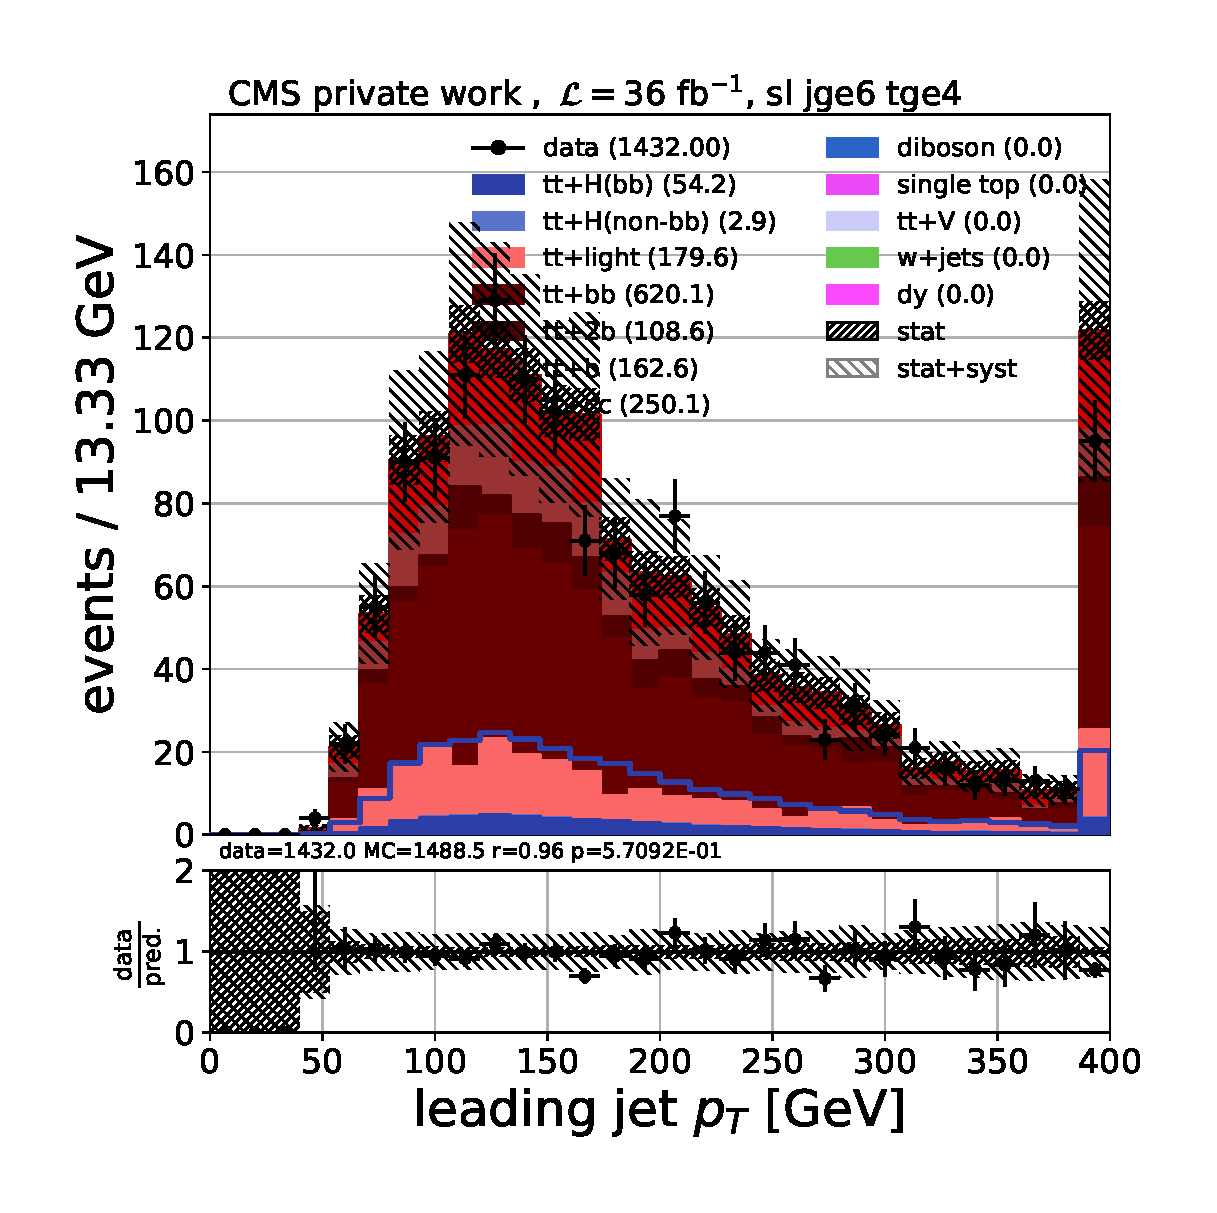
\includegraphics[width=0.4\textwidth]{figures/jetsByPt_0_pt.pdf}} 
\subfloat[fig 2]{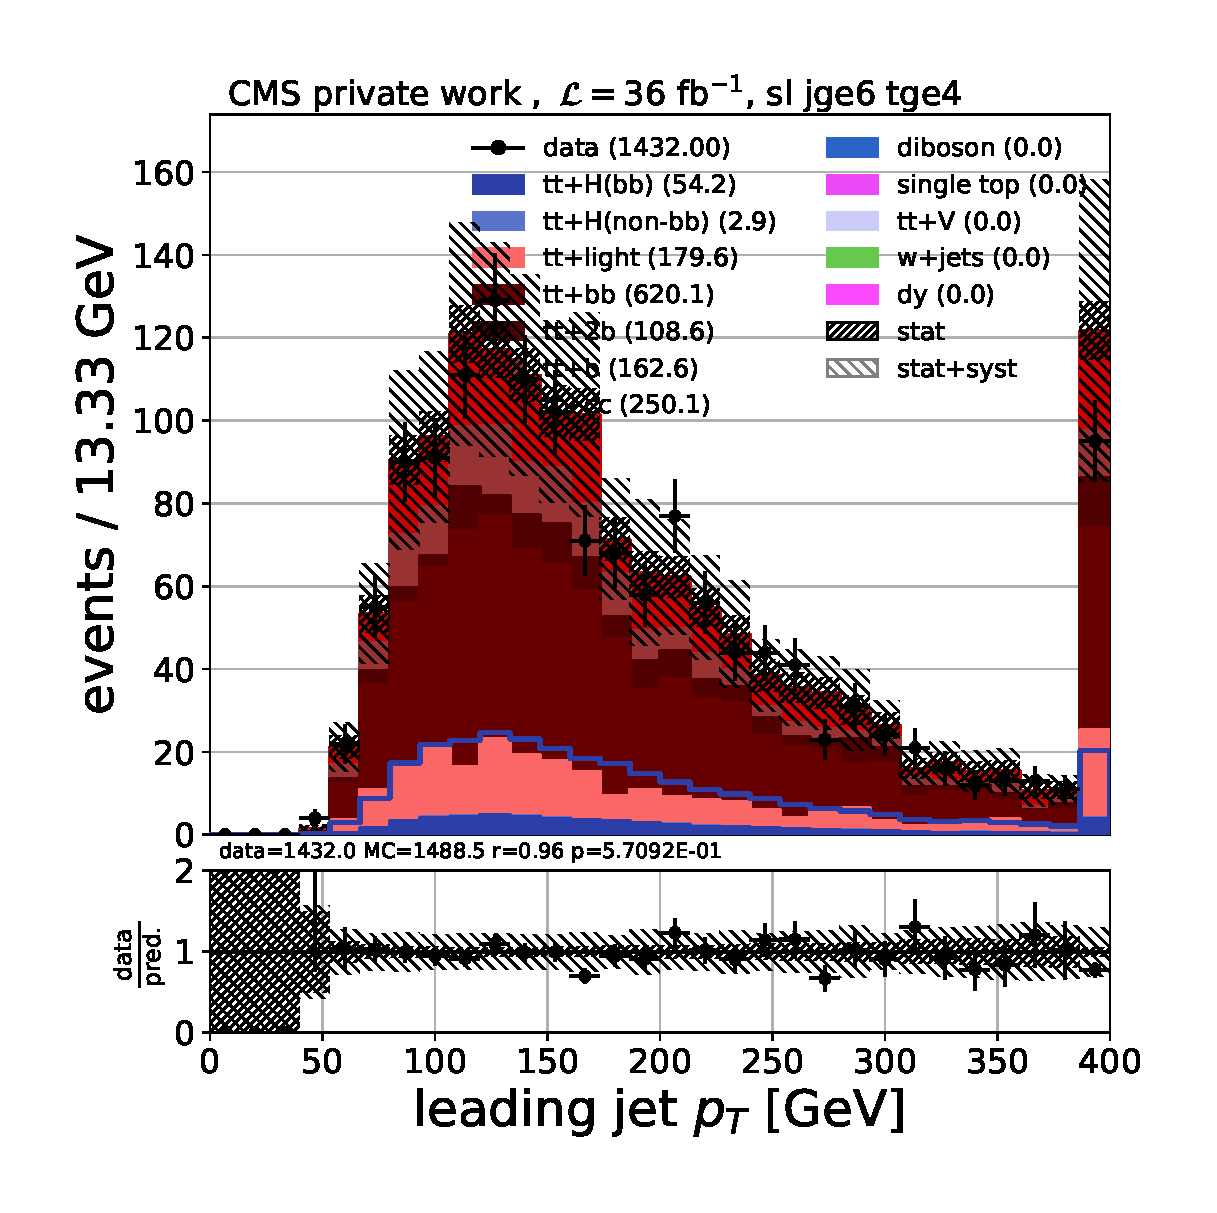
\includegraphics[width=0.4\textwidth]{figures/jetsByPt_0_pt.pdf}}\\
\caption{MEM assumptions.}
\label{fig:mem_assumptions}
\end{centering}
\end{figure}


\subsubsection{Integration}
\label{sec:mem_integration}

The MEM is implemented as a dedicated code in C++, relying on the \texttt{OpenLoops} C++ interface for the evaluation of the hard scattering amplitude. \texttt{ROOT} is used for numerical Lorentz algebra and \texttt{CLING} for interfacing the code to Python. The PDFs are evaluated using the \texttt{cteq66} set via the \texttt{LHAPDF} package. The numerical integration routines rely on the \texttt{VEGAS} algorithm that uses multiple passes to refine the integration grid, with the maximal number of evaluations tuned for approximately $<2.5 \dots 5\%$ numerical accuracy on the integral, suitable for use in a discriminator. We use the \texttt{CUBA} package for numerical integration, as it supports vector-valued integrands. The distribution of expected numerical accuracy is shown on \cref{fig:mem_numerical_accuracy} and illustrates the convergence of the numerical integration. Transfer functions can be provided in a flexible parametrisation using \texttt{ROOT}, however, as described in \cref{sec:mem_optimization}, we have also provided faster, optimized versions of the chosen Gaussian transfer functions. 

\fix Describe integration boundaries.

\begin{figure}
\begin{centering}
\subfloat[fig 1]{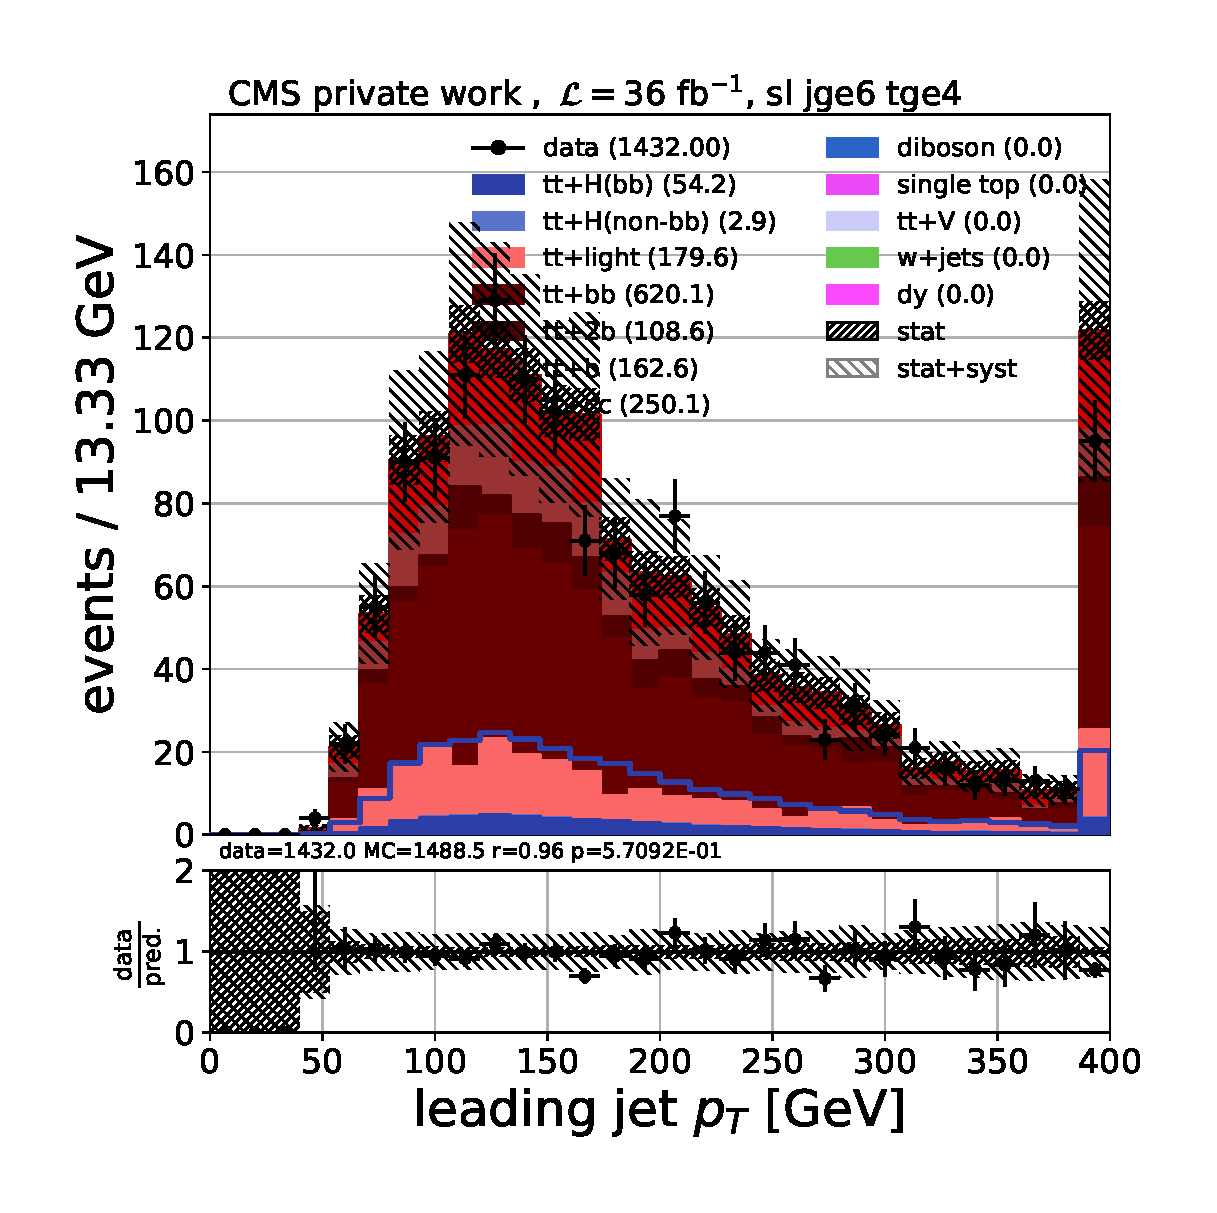
\includegraphics[width = 0.4\linewidth]{figures/jetsByPt_0_pt.pdf}} 
\subfloat[fig 2]{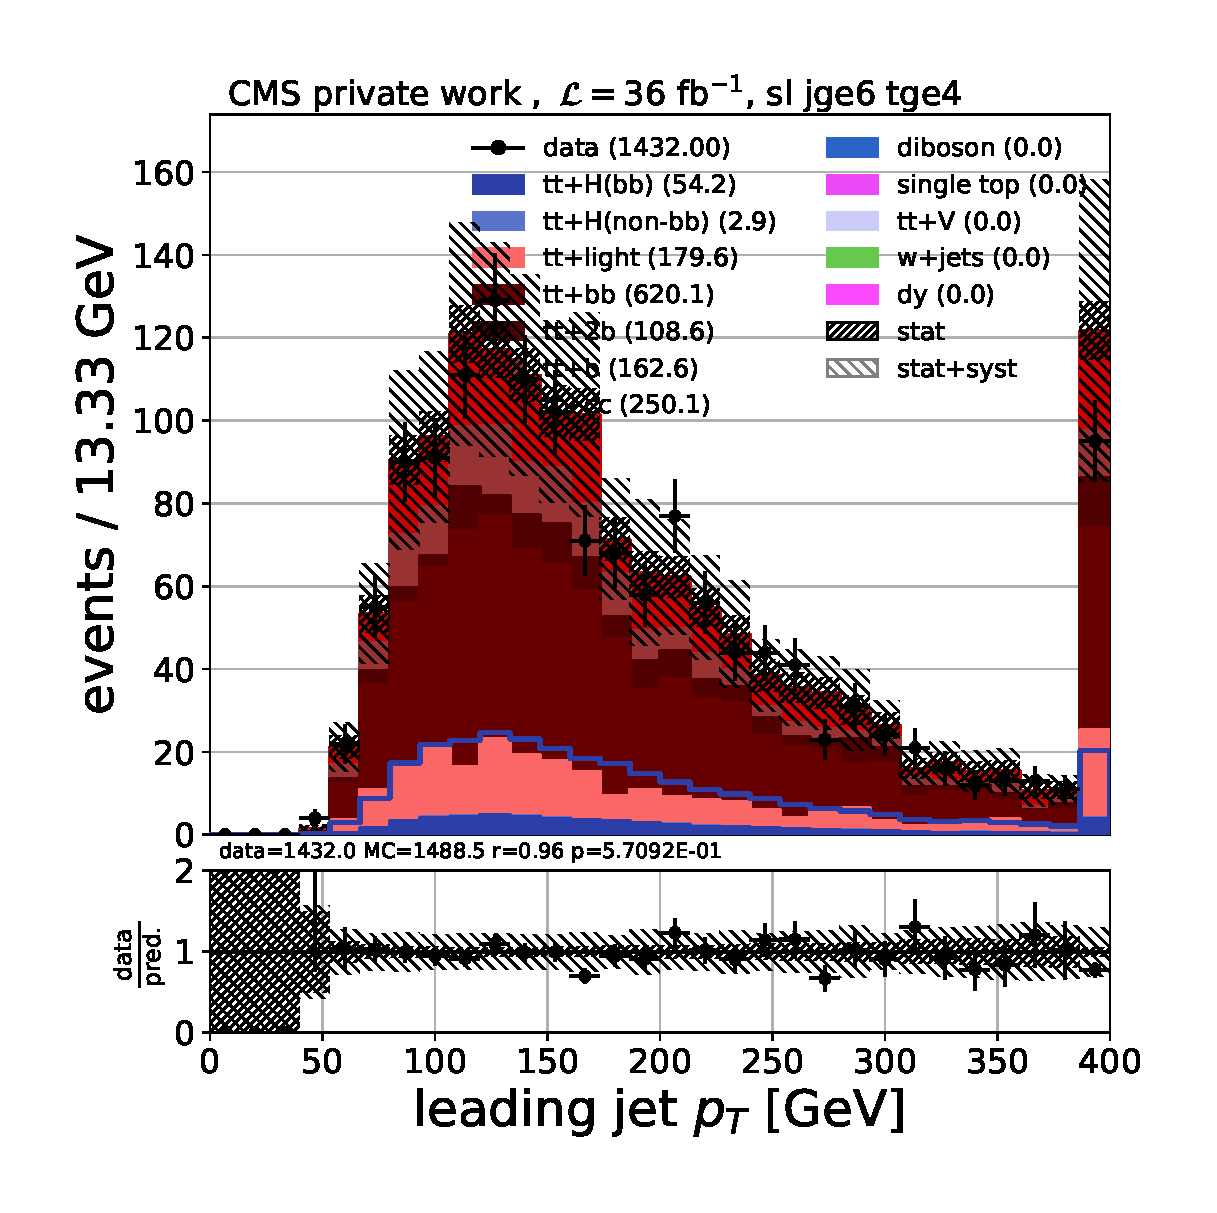
\includegraphics[width = 0.4\linewidth]{figures/jetsByPt_0_pt.pdf}}\\
\caption{MEM assumptions.}
\label{fig:mem_numerical_accuracy}
\end{centering}
\end{figure}

\subsubsection{Profiling and optimisation}
\label{sec:mem_optimization}

In order to optimize the MEM code, we have used the \texttt{igprof} sampling profiler tool to analyze the computational budget spent in various subroutines of the code. In general, we find    
that the overwhelming majority of time is spent within the integrand, out of which about 40\% is spent computing the transfer functions, 35\% is spent evaluating the scattering amplitude of the hard process, 10\% of computing the PDFs and about 10\% on manipulating the phase space volume. The evaluation of the transfer functions at a single phase space point is about an order of magnitude faster than the scattering amplitude. In order to achieve this ratio, we implemented the transfer functions explicitly as optimized C++ functions, instead of relying on a more generic approach using symbolic functions supported in ROOT. Additionally, as we have seen that a large part of time optimising the integration grid is spent in the exponential tails of the transfer function, we have used a piecewise exponential function that is suppressed far in the tails.

Currently, the MEM algorithm as implemented here can only be run on standard x86 CPU architectures. Although it has been shown that GPUs may offer strong parallelization benefits in evaluating the integral, it would be necessary to completely port and optimize the \texttt{OpenLoops} toolset on the GPU in a significant engineering effort\cite{Schouten:2014yza}, furthermore, GPU clusters are currently not commonplace in the WLCG.

\subsubsection{Computational budget}
\label{sec:mem_computational}
In this section, we present a feasibility estimation on using the MEM in a Run II analysis. This is necessary in order to predict the amount of computing resources that will be required. The computing time depends strongly on the number of permutations and integration variables needed for a given interpretation and event topology, as well as the total number of MC simulated events that are needed for the analysis.

\begin{table}[h!]
\begin{center}
\caption{The CPU budget of the MEM. \fix}
\label{tab:mem_cpu_budget}
\begin{tabular}{ccccc}
\hline
category & interpretation & average time & events & total \\
\hline
$1\ell6\mathrm{j}4\mathrm{t}$ & $2_{\mathrm{W}} 2_{\mathrm{h}} 2_{\mathrm{t}}$ & 60 CPUs/ev & 12044 ev & 100 CPUh \\
$1\ell7\mathrm{j}4\mathrm{t}$ & $2_{\mathrm{W}} 2_{\mathrm{h}} 2_{\mathrm{t}}$ & 60 CPUs/ev & 12044 ev & 100 CPUh \\
$1\ell\ge8\mathrm{j}4\mathrm{t}$ & $2_{\mathrm{W}} 2_{\mathrm{h}} 2_{\mathrm{t}}$ & 60 CPUs/ev & 12044 ev & 100 CPUh \\
$1\ell\ge5\mathrm{j}4\mathrm{t}$ & $1_{\mathrm{W}} 2_{\mathrm{h}} 2_{\mathrm{t}}$ & 60 CPUs/ev & 12044 ev & 100 CPUh \\
$1\ell\ge4\mathrm{j}4\mathrm{t}$ & $0_{\mathrm{W}} 2_{\mathrm{h}} 2_{\mathrm{t}}$ & 60 CPUs/ev & 12044 ev & 100 CPUh \\

\hline
\hline
\end{tabular}
\end{center}
\end{table}

\subsubsection{Uncertainties}
\label{sec:mem_uncertainties}

When using the MEM in a realistic experimental analysis, we need to evaluate the effect of systematic uncertainties on the MEM. In general, uncertainties modify the observables $\vec{y} \rightarrow \vec{y}^*$, for example the jet energies may be modified by uncertainties in the jet energy scale calibration. The naive approach to estimate the sensitivity of the discriminator would be to recompute the MEM discriminator weights $P(\vec{y}) \rightarrow P(\vec{y}^*)$. However, this turns out to be impractical, since the number of individual variations that need to be considered can easily reach $\mathcal{O}(10^2)$ and it is not realistic or practical to expend two orders of magnitude more computational resources.
In order to improve the situation, we first note that the variations are generally small, such that $\vec{y}^* \simeq \vec{y} + \delta \vec{y}$. Therefore, the numerical integration described in section \cref{sec:mem_implementation} would be performed on almost the same phase space, with a very similar integration grid.

Furthermore, we see from \cref{eq:definition} that the observables enter the definition of the MEM probability primarily through the transfer functions $W(\vec{y} | \vec{p})$ and affect the integration volume only secondarily. The most computationally costly part in the integrand is the evaluation of the LO scattering amplitudes for the hard process. Therefore, if we can promote the integrand to a vector-valued quantity, such that
\begin{equation}
|\mathcal{M}(\vec{p})|^2 W(\vec{y} | \vec{p}) \rightarrow |\mathcal{M}(\vec{p})|^2  \begin{pmatrix}
  W(\vec{y} | \vec{p}) \\
  W(\vec{y} + \delta \vec{y}_1 | \vec{p}) \\
  \dots \\
  W(\vec{y} + \delta \vec{y}_n | \vec{p})
 \end{pmatrix},
\end{equation}
the integration of the nominal and variated weight can be performed in a single pass using a a grid optimised for the whole integration. We test this approach by comparing the variation evaluated using vector integration to the full computation. As we wish to estimate the sensitivity of the analysis to this uncertainty, it is sufficient if the approximated variation has the same magnitude and direction as the true variation.

Additional complexity is introduced due to variations in the uncertainties possibly changing the topology of the reconstructed final state, as scaling jet energies down may cause jets to migrate under the experimental threshold $p_{T\mathrm{cut}}$. In order to account for this, in case a particular variation $\vec{y} + \delta \vec{y}_n$ changes the reconstructed final state, the MEM is still recomputed from scratch.

\subsubsection{MEM on the WLCG}

From \cref{sec:mem_computational} it is apparent that it is necessary to compute the MEM on distributed systems in order to have a reasonable turn-around time for the analysis. Therefore, we have parallelized the workflow both on the level of a computing cluster using \texttt{grid-control} and the WLCG using \texttt{CRAB}. On the WLCG, we have thus been able to take advantage of CMS computing resources opportunistically and have demonstrated that the MEM as implemented here is able to run on a wide range of data centers on a planetary scale. For this, we relied on \texttt{CMSSW} to provide a consistent environment along with user-provided external dependencies such as \texttt{OpenLOOPS}. We integrated the MEM into a multi-step workflow that produced the final analysis data sets directly from CMS MiniAOD in a single pass. This way, we were able to benefit from load balancing using data locality in CMS and reduced the number of manual intermediate steps and data management which can be error prone.
% asdasd \ttH

\subsection{Expected performance}
We demonstrate the expected performance of the MEM on a MC simulation sample of \ttH and \ttbar+jets. First, on \cref{fig:mem_proba}, we verify that the signal and background probabilities indeed behave as expected on their respective MC simulations.

\begin{figure}
\begin{centering}
\subfloat[MEM probability for the \ttH hypothesis.]{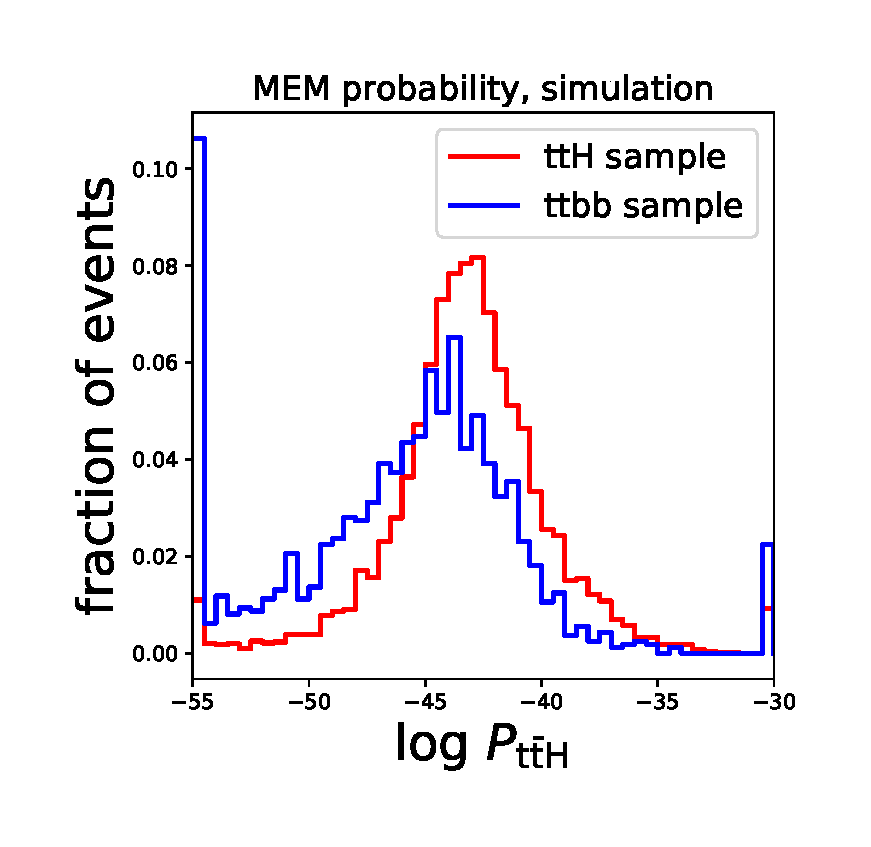
\includegraphics[width = 0.5\textwidth]{figures/mem_proba_tth.pdf}} 
\subfloat[MEM probability for the \ttbb hypothesis]{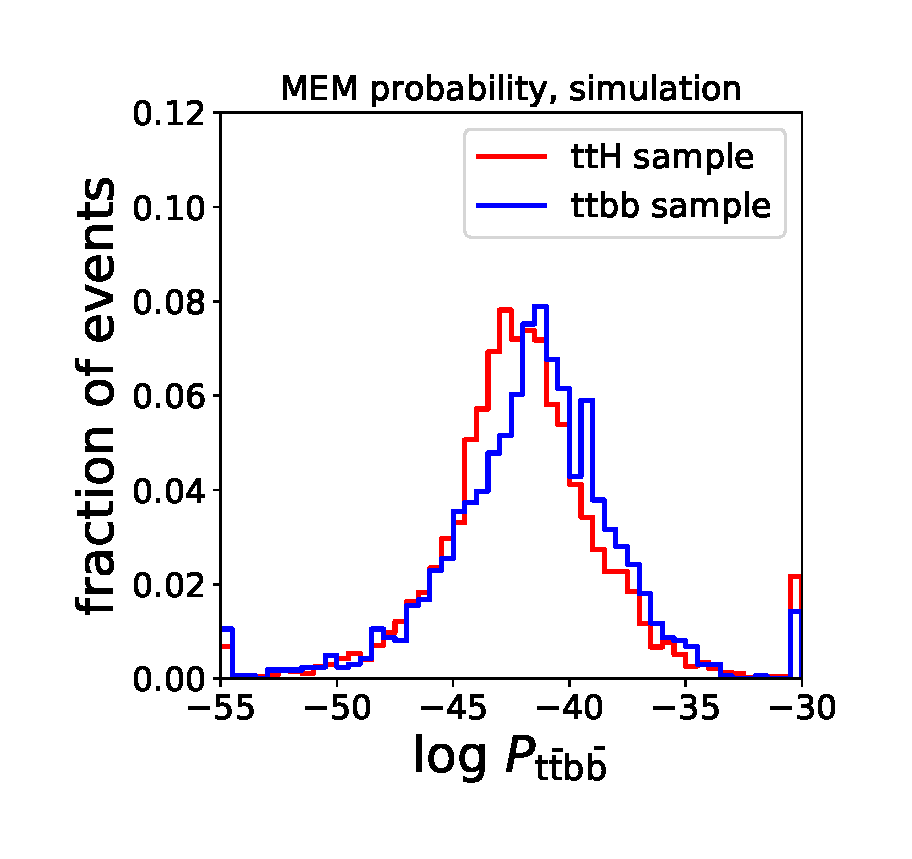
\includegraphics[width = 0.5\textwidth]{figures/mem_proba_ttbb.pdf}}\\
\caption{The expected distribution of the signal probability $P_{\ttHbb}$ and the background probability $P_{\ttbb}$ on MC simulation. We see that for the signal sample, the signal probability is on average higher than the background probability, and vice versa for the background. Here, we have selected events with exactly 1 isolated lepton, at least 6 jets, out of which 4 must be b tagged. Furthermore, the jets are required to be matched to quarks from the corresponding hard interaction on generator level.}
\label{fig:mem_proba}
\end{centering}
\end{figure}

\begin{figure}
\begin{centering}
\subfloat[fig 2]{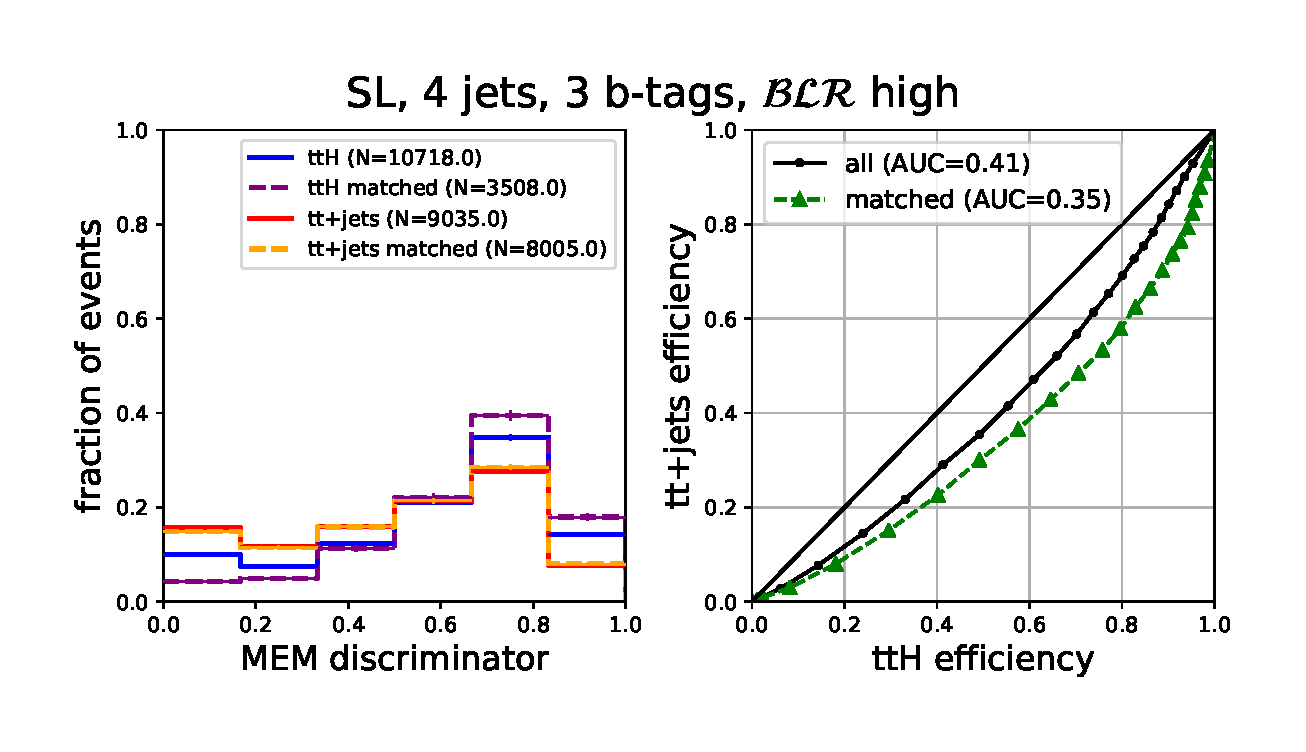
\includegraphics[width = 1.0\textwidth]{figures/mem_sl_j4_t3_blrH.pdf}}\\
\subfloat[fig 1]{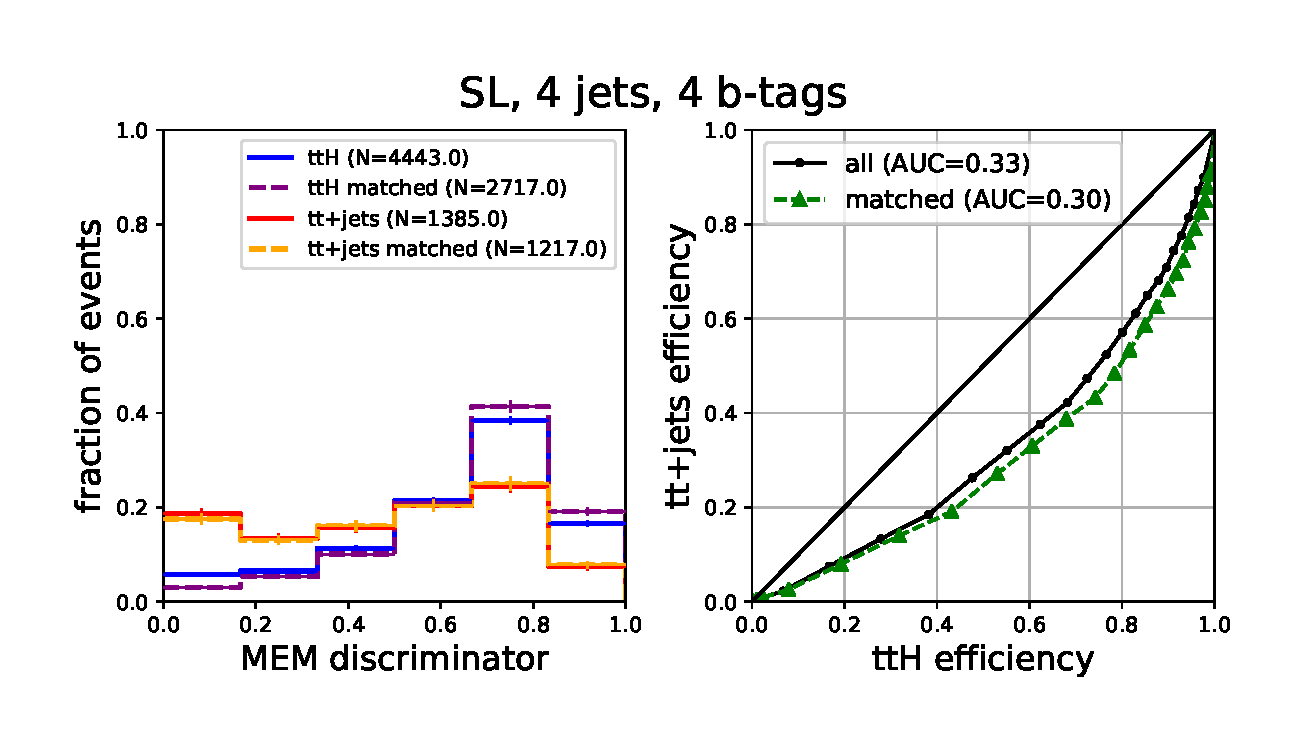
\includegraphics[width = 1.0\textwidth]{figures/mem_sl_j4_t4.pdf}}\\
\caption{Add your own figures before compiling}
\label{fig:some_example}
\end{centering}
\end{figure}

\begin{figure}
\begin{centering}
\subfloat[fig 2]{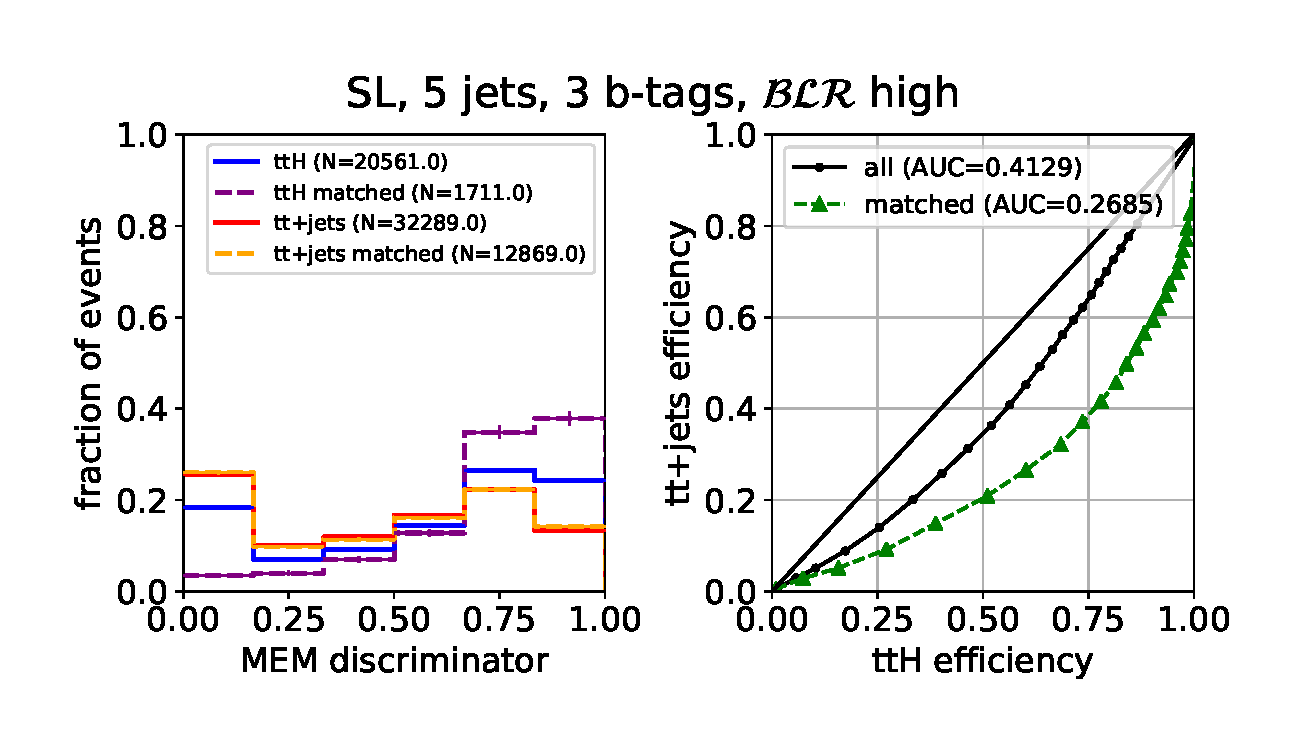
\includegraphics[width = 1.0\textwidth]{figures/mem_sl_j5_t3_blrH.pdf}}\\
\subfloat[fig 1]{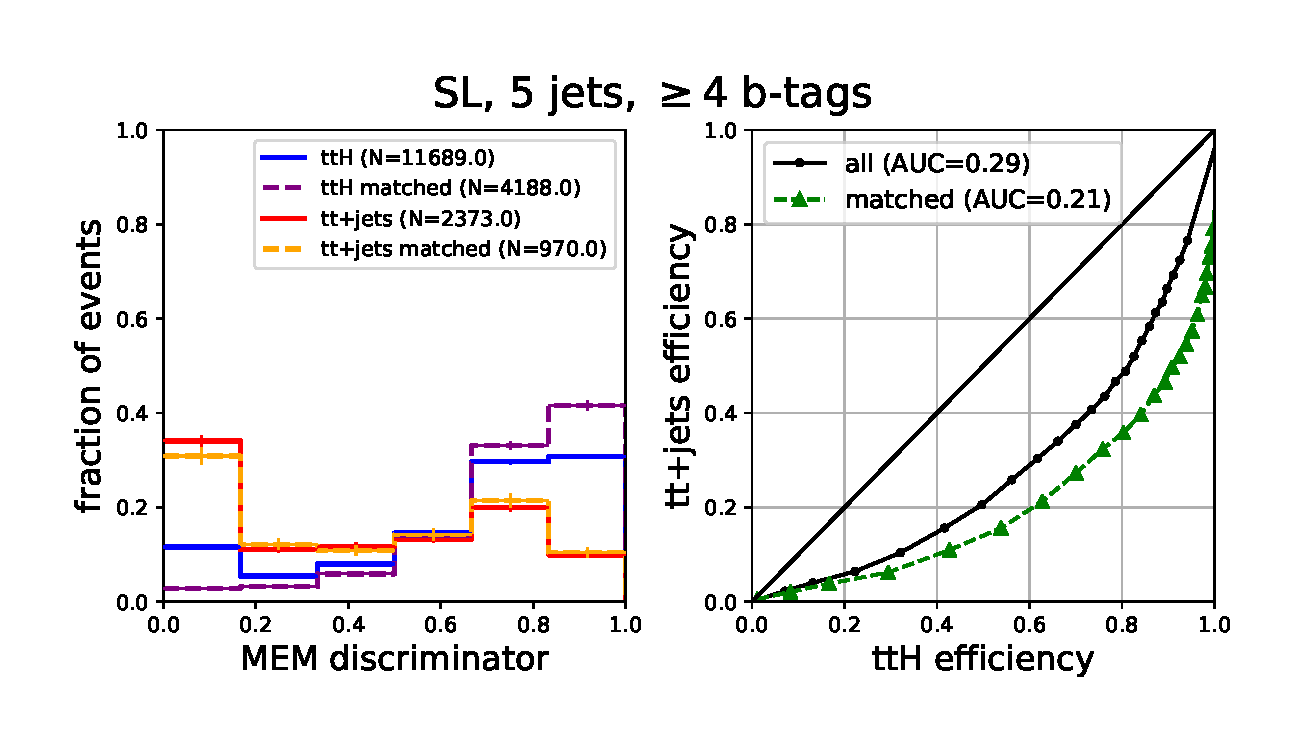
\includegraphics[width = 1.0\textwidth]{figures/mem_sl_j5_tge4.pdf}}\\
\caption{Add your own figures before compiling}
\label{fig:some_example}
\end{centering}
\end{figure}

\begin{figure}
\begin{centering}
\subfloat[fig 1]{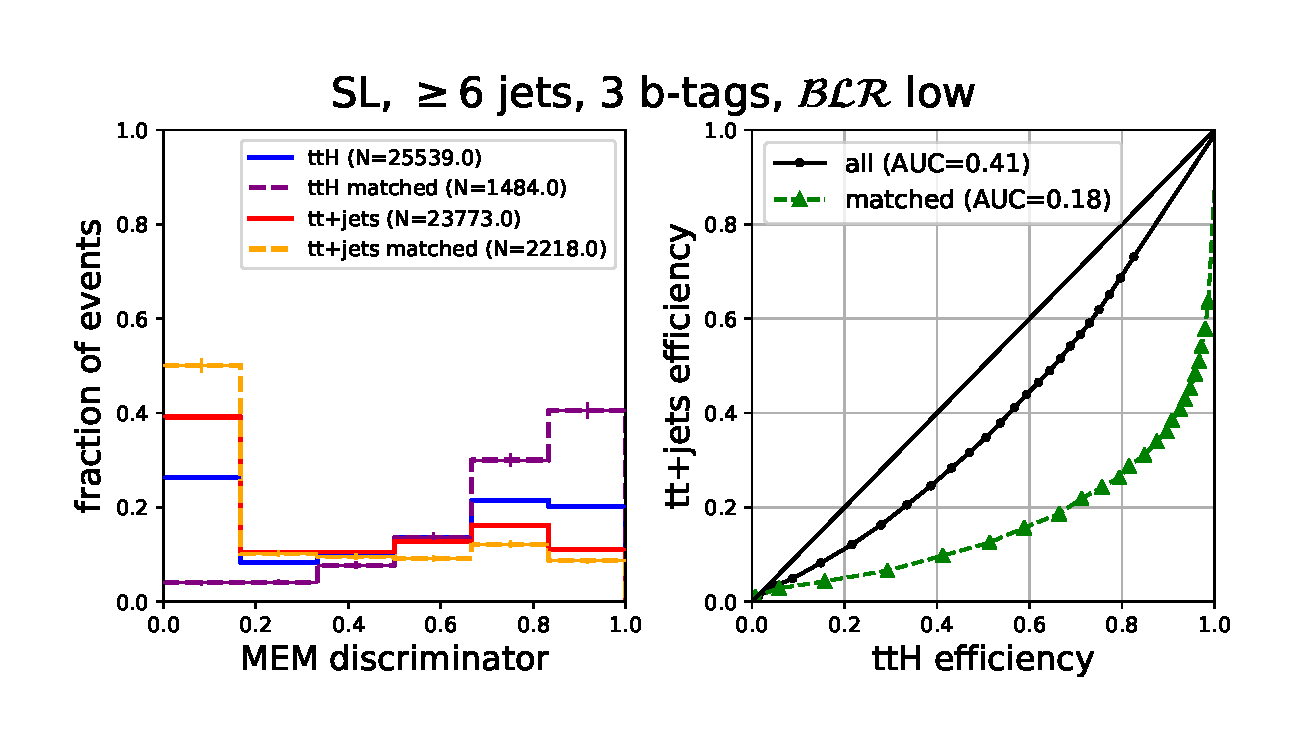
\includegraphics[width = 1.0\textwidth]{figures/mem_sl_jge6_t3_blrL.pdf}}\\
\subfloat[fig 2]{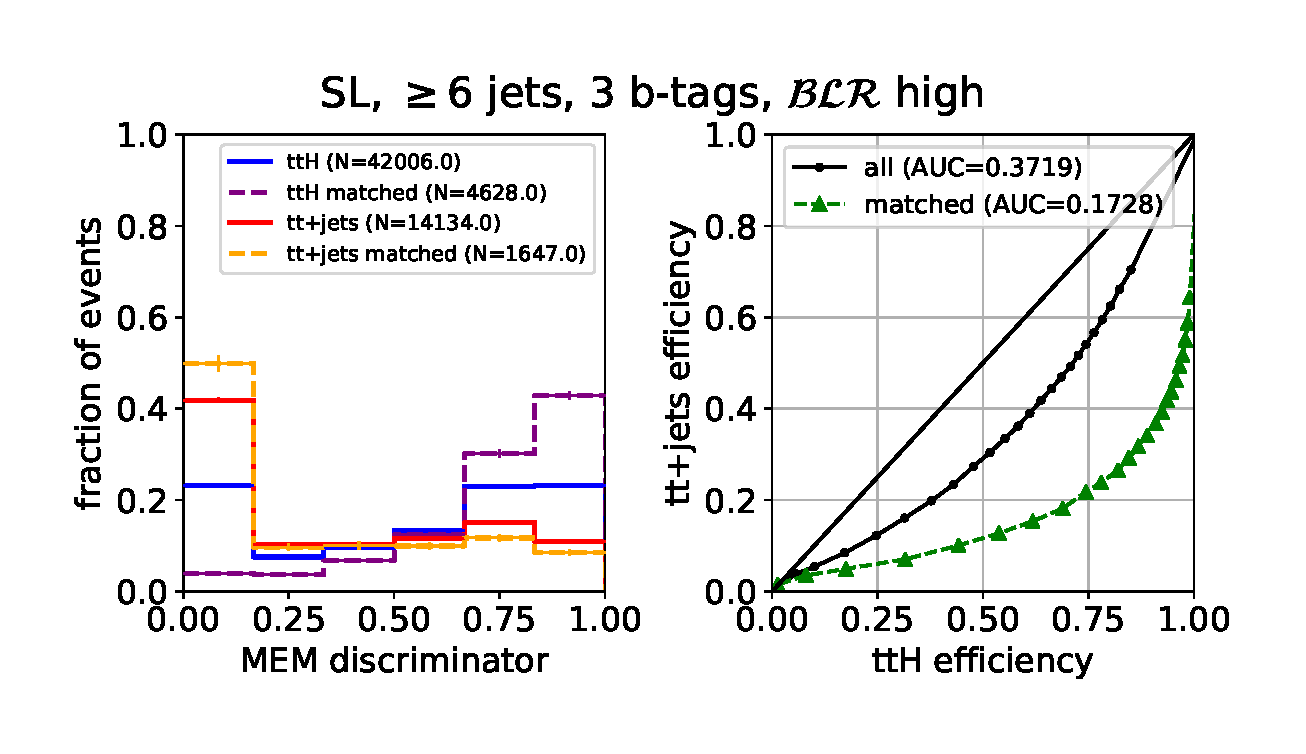
\includegraphics[width = 1.0\textwidth]{figures/mem_sl_jge6_t3_blrH.pdf}}\\
\caption{Add your own figures before compiling}
\label{fig:some_example}
\end{centering}
\end{figure}

\begin{figure}
\begin{centering}
\subfloat[fig 3]{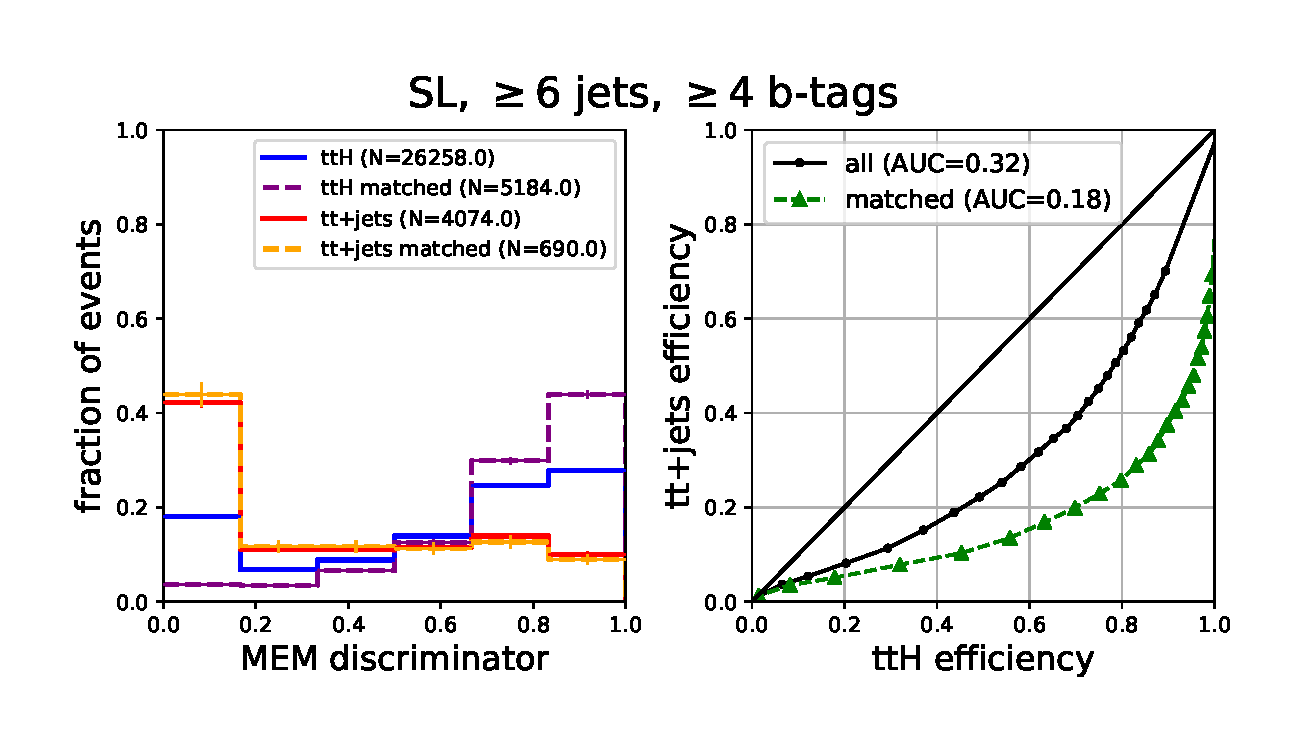
\includegraphics[width = 1.0\textwidth]{figures/mem_sl_jge6_tge4.pdf}}\\
\subfloat[fig 4]{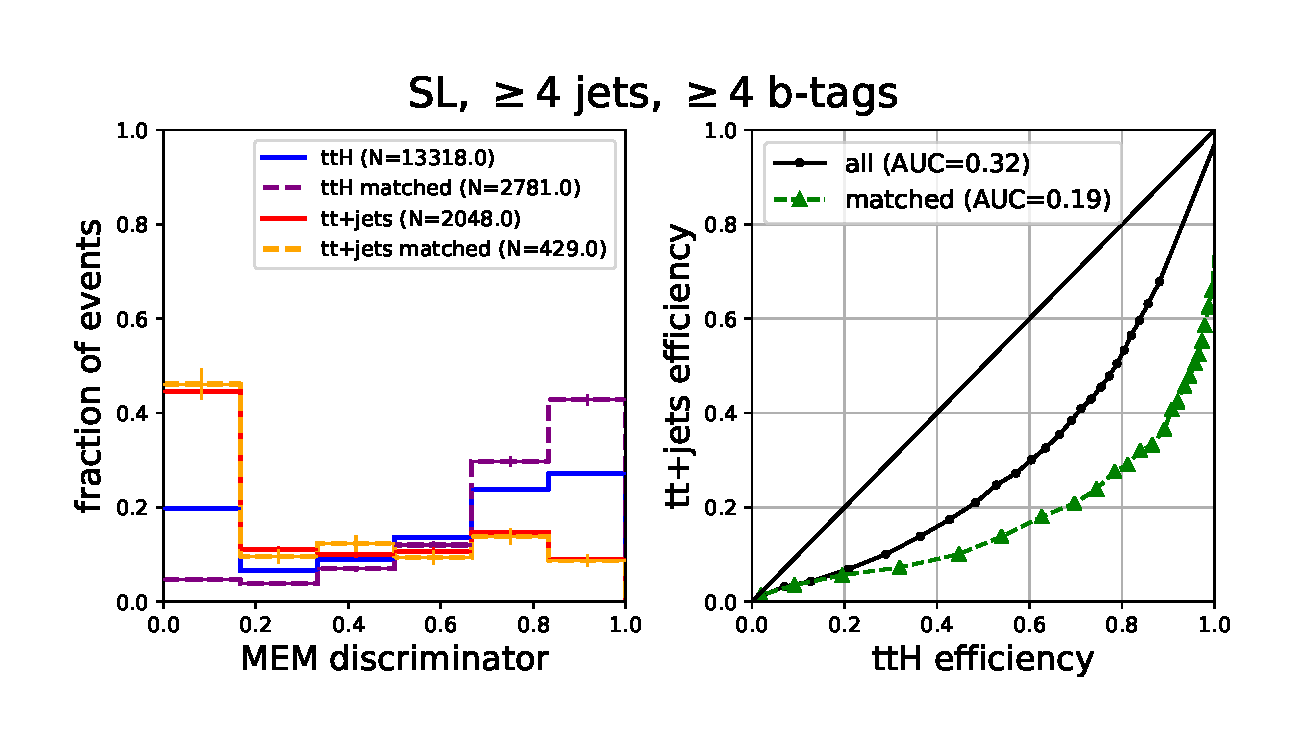
\includegraphics[width = 1.0\textwidth]{figures/mem_sl_jge7_tge4_7jet.pdf}}\\ 
\caption{Add your own figures before compiling}
\label{fig:some_example}
\end{centering}
\end{figure}


% \begin{figure}
% \begin{centering}
% \subfloat[fig 1]{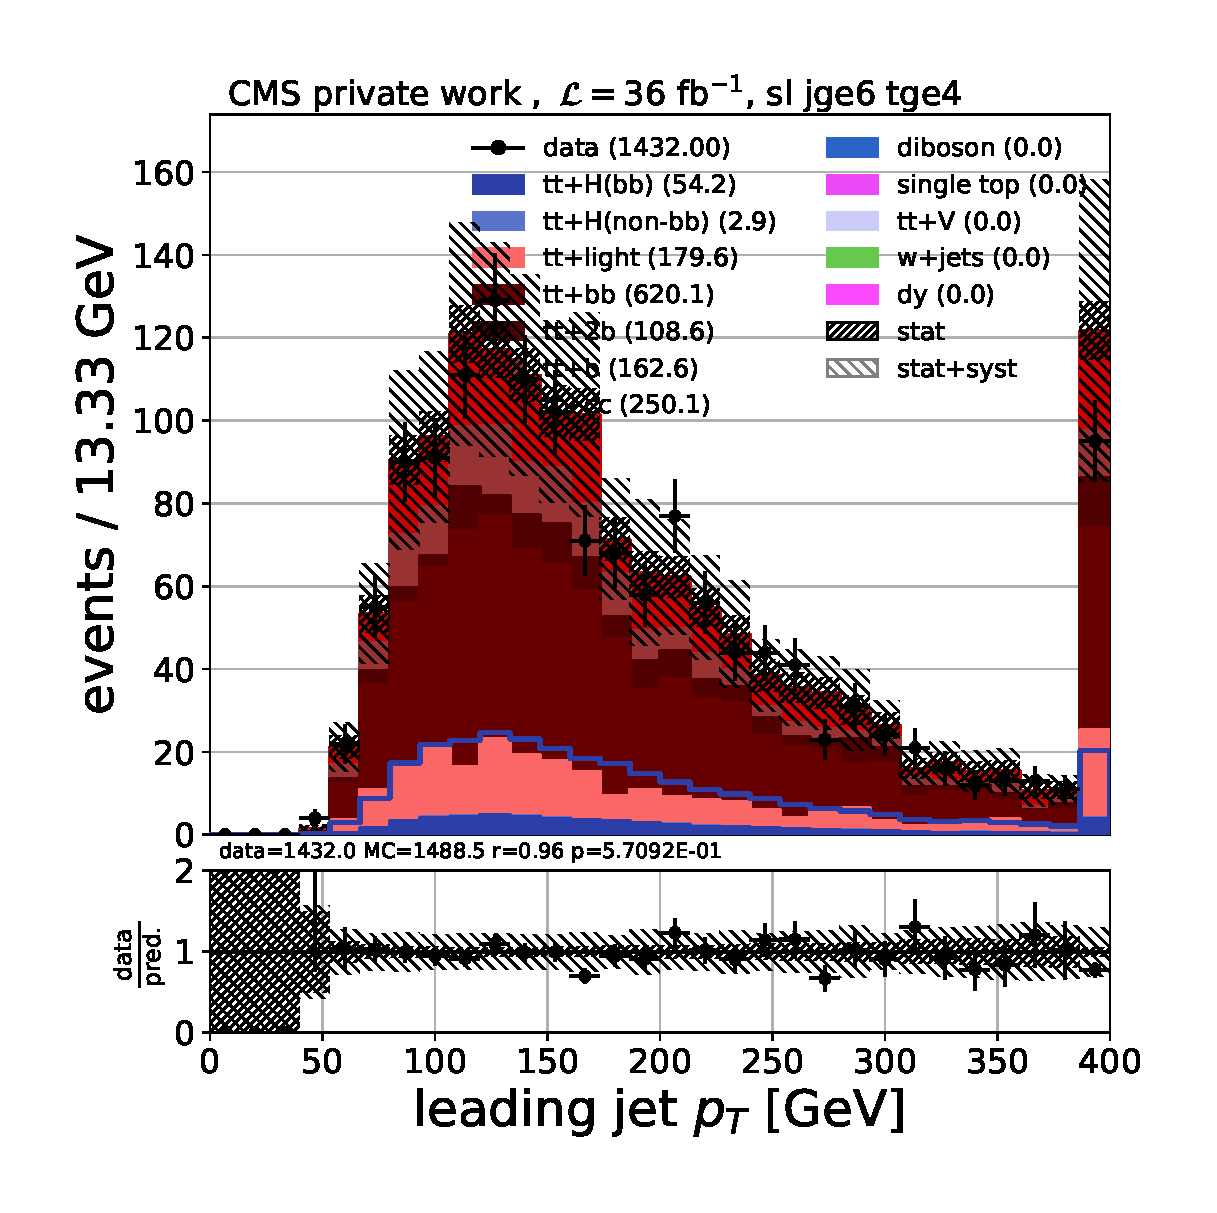
\includegraphics[width = 0.4\linewidth]{figures/jetsByPt_0_pt.pdf}} 
% \subfloat[fig 2]{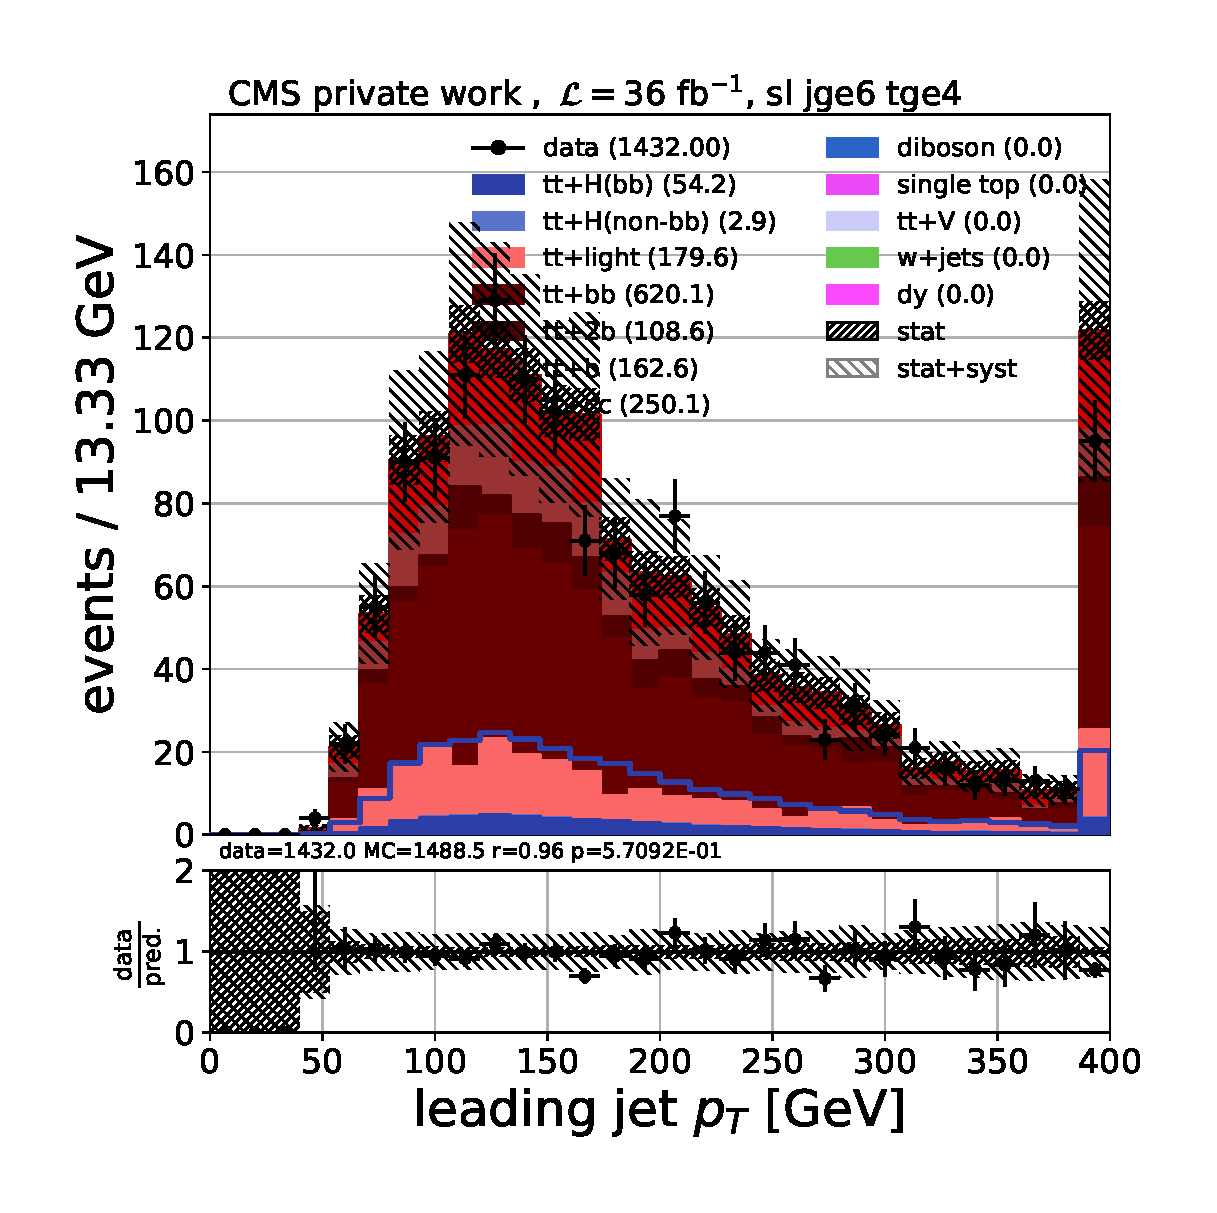
\includegraphics[width = 0.4\linewidth]{figures/jetsByPt_0_pt.pdf}}\\
% \subfloat[fig 3]{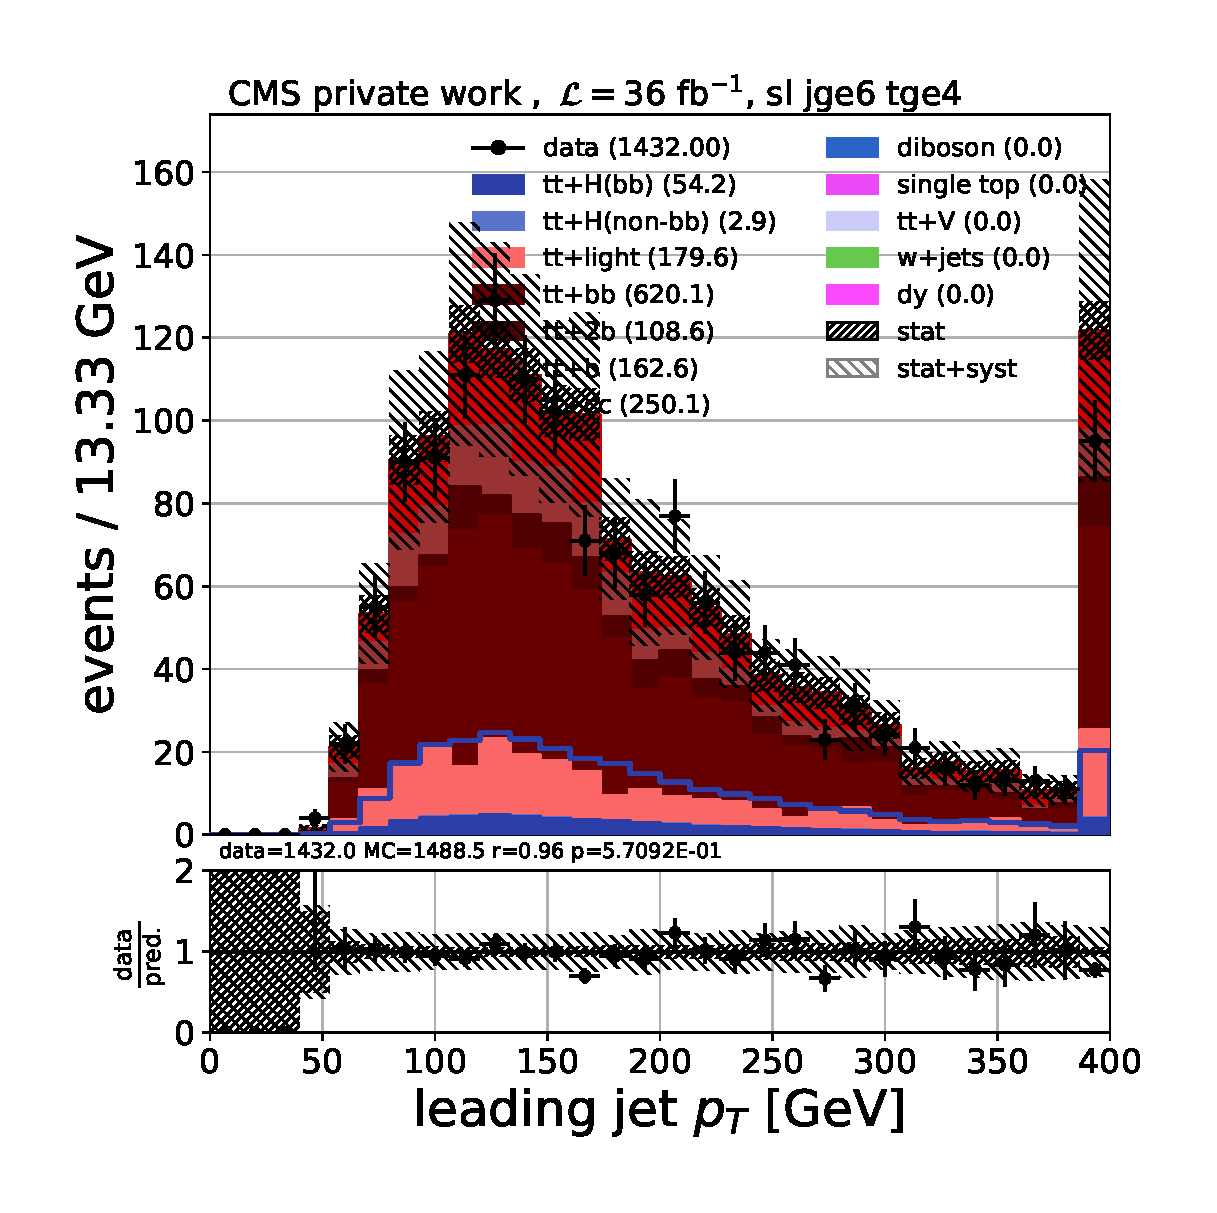
\includegraphics[width = 0.4\linewidth]{figures/jetsByPt_0_pt.pdf}}
% \subfloat[fig 4]{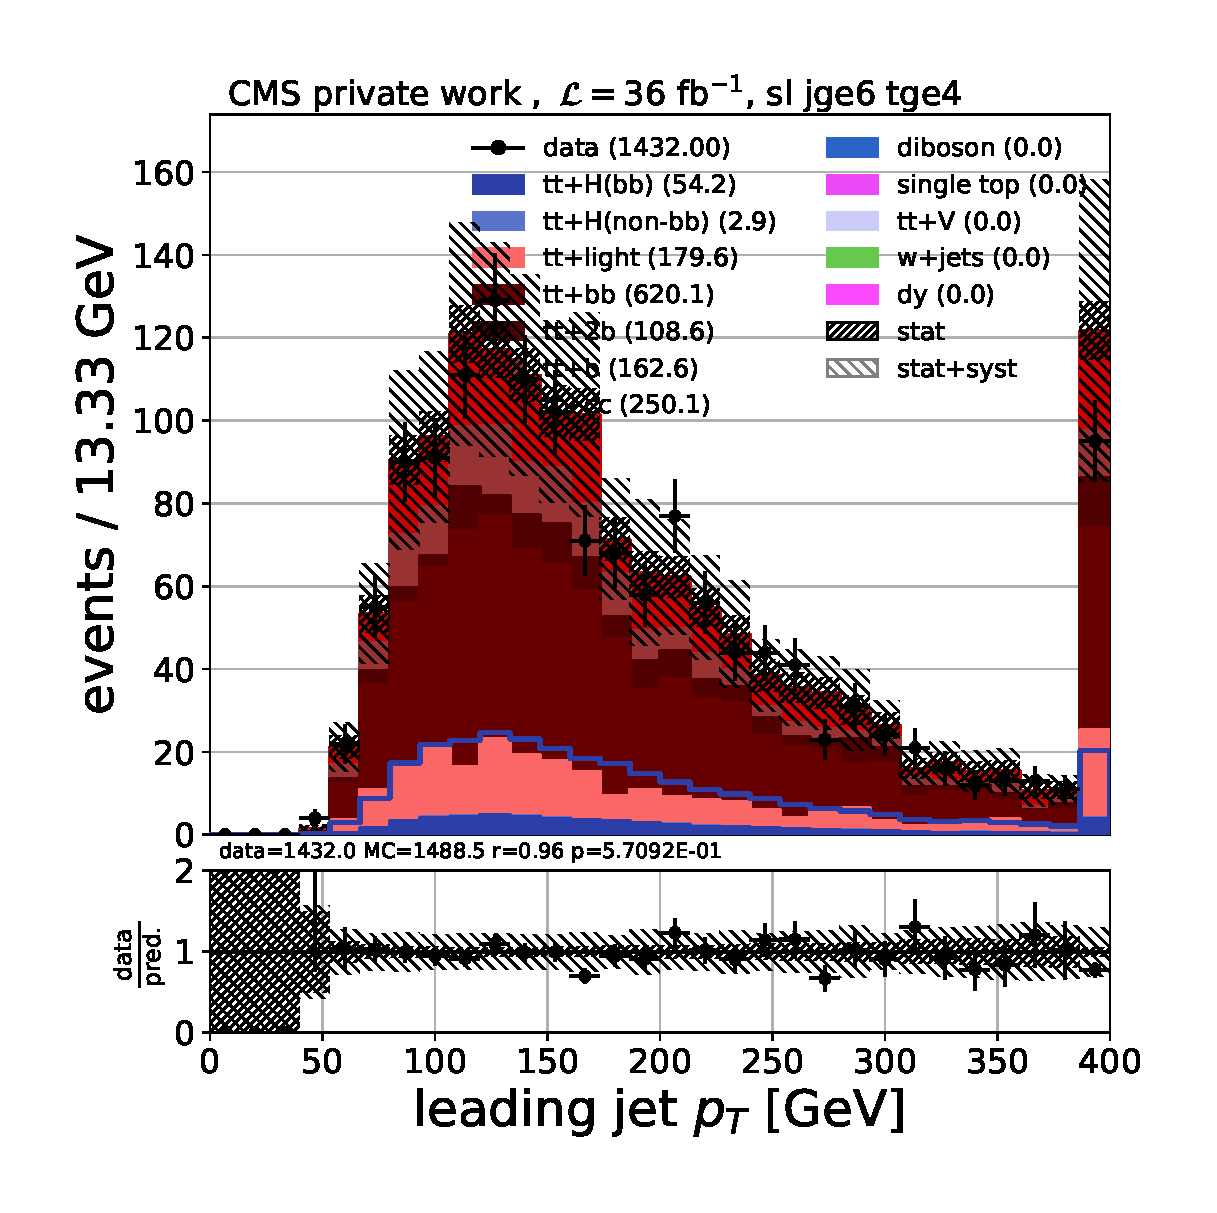
\includegraphics[width = 0.4\linewidth]{figures/jetsByPt_0_pt.pdf}} 
% \caption{Add your own figures before compiling}
% \label{fig:some_example}
% \end{centering}
% \end{figure}

% On \cref{fig:some_example} bla bla